\documentclass[a4paper, 14pt]{extarticle}

\usepackage{generalPreamble}
\usepackage{reportFormat}

\begin{document}

\begin{titlepage}
    \centering
    {\bfseries
        \uppercase{
            Минобрнауки России \\
            Санкт-Петербургский государственный \\
            Электротехнический университет \\
            \enquote{ЛЭТИ} им. В.И.Ульянова (Ленина)\\
        }
        Кафедра МО ЭВМ

        \vspace{\fill}
        \uppercase{Лабораторная работа №1} \\
        по дисциплине \enquote{Криптография и защита информации} \\
        Тема: Изучение классических шифров средствами RailFence, Scytale, Caesar
    }

    \vspace{\fill}
    \begin{tabularx}{0.8\textwidth}{l X c r}
        Студент гр. 6304 & & \underline{\hspace{3cm}} & Корытов П.В.\\
        Преподаватель & & \underline{\hspace{3cm}} & Племянников
    \end{tabularx}

    \vspace{1cm}
    Санкт-Петербург \\
    \the\year{}
\end{titlepage}

\newpage

\section*{Цель работы}
Исследовать шифры Rail Fence, Scytale, Caesar и получить практические навыки работы с ними, в том числе и в программногом продукте Cryptool 1 и 2.

\section{Шифр Rail Fence}
\subsection{Задание}
\begin{enumerate}
    \item Найти шифр в CrypTool 1: Encrypt/Decrypt-> Symmetric (Classis).
    \item Создать файл с открытым текстом, содержащим последовательность цифр.
    \item Запустить шифр и выполнить зашифровку и расшифровку созданного текста несколько раз.
    \item Установить, как влияют на шифрование параметры Number of Rows и Offset.
    \item Зашифровать и расшифровать текст, содержащий только фамилию (транслитерация латиницей) вручную и с помощью шифра при Number of Rows>2, Offset≥2. Убедиться в совпадении результатов.
    \item Создайте шифровку для варианта Offset=0 и Number of Rows≤ и передайте коллеге слева для расшифровки.
    \item Определите ключ методом ``грубой сил'' и расшифруйте полученный от коллеги шифротекст.
\end{enumerate}
\subsection{Описание шифра}
В шифре Изгороди открытый текст разбивается на определенное количество строк. В каждой строке поочередно записывается одна буква подобно изгороди, зашифрованный текст составляется при чтении строки за строкой. Например, при разбиении открытого текста ``0123456789'' на 3 строки шифрование выглядит следующим образом:

\begin{tabularx}{0.8\textwidth}{XXXXXXXXXXXX}
\multicolumn{10}{c}{Разбиение на строки} &  & Шифротекст \\
0 &  &  &  & 4 &  &  &  & 8 &  &  &  \\
 & 1 &  & 3 &  & 5 &  & 7 &  & 9 & =\textgreater{} & 0481357926 \\
 &  & 2 &  &  &  & 6 &  &  &  &  & 
\end{tabularx}

Для увеличения криптостойкости используют смещение. Пример для смещения 2:

\begin{tabularx}{0.8\textwidth}{XXXXXXXXXXXXX}
\multicolumn{10}{c}{Разбиение на строки} &  &  & Шифротекст \\
--- &  &  &  & 3 &  &  &  & 7 &  &  &  &  \\
 & --- &  & 2 &  & 4 &  & 6 &  & 8 &  & =\textgreater{} & 2613579048 \\
 &  & 1 &  &  &  & 5 &  &  &  & 9 &  & 
\end{tabularx}

\section{Шифр ``Сцитала'' (Scytale)}
В криптографии сцитала, известный также как шифр Древней Спарты, представляет собой прибор, используемый для осуществления перестановочного шифрования. Прибор состоит из цилиндра и узкой полоски пергамента, обматывавшейся вокруг него по спирали, на которой писалось сообщение. Иллюстрация, демонстрирующая работу данного шифра представлена на рисунке~\ref{img:theory:1}.

\begin{figure}[h]
    \centering
    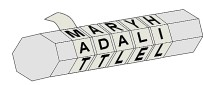
\includegraphics[width=0.4\textwidth]{img/S004.jpg}
    \caption{Иллюстрация шифра Сцитала}%
    \label{img:theory:1}
\end{figure}

Для расшифровки использовался цилиндр такого же диаметра, на который наматывался пергамент, чтобы прочитать сообщение.

\subsection{Шифр Цезаря (Caesar)}

Шифр Цезаря — один из древнейших шифров. Шифр назван в честь римского императора Гая Юлия Цезаря, использовавшего его для секретной переписки.

\begin{itemize}
    \item Заменим буквы алфавита числами соответствующими их порядковым номерам в алфавите $0, 1, \ldots, n-1$.
    \item Представим символы открытого текста $P_i$ и шифротекста $C_i$
    \item Выбираем в качестве ключа числа $k$
    \item Шифрование: $C_i = (P_i + k) \bmod n$ 
    \item Расшифровка: $ P_i = (C_i - k) \bmod n $
\end{itemize}
\end{document}
